%!TEX root = ./template-skripsi.tex
%-------------------------------------------------------------------------------
%                            BAB IV
%               		HASIL DAN PEMBAHASAN
%-------------------------------------------------------------------------------

\chapter{HASIL DAN PEMBAHASAN}

Pada penelitian tugas akhir ini, pengujian sistem deteksi \emph{anomali traffik} dila-
kukan dengan mengukur detection rate, accuracy. Data yang digunakan dalam pe-
ngujian berjumlah 5 juta dataset normal ,5 juta dataset serangan DDos ,5 juta dataset
serangan Brute Force ,5 juta dataset serangan Scanning. Pengujian pada peneltian
ini akan menghitung akurasi deteksi setiap serangan , kecepatan waktu komukiasin
antara server dan telegram, dan kapasitas memory yang digunakan oleh server dalam
menjalankan aplikasi ini.

	\section{Kebutuhan Pengujian}
		Data yang digunakan pada pengujian merupakan sebagian data dari dataset
		hasil scapy preprocessing yang telah telah dijadikan sebuah \emph{rule} dengan data seba-
		nyak masing masing 5 juta dataset . Data yang digunakan untuk proses training deci-
		sion tree menggunakan data dari hasil \emph{capturing traffik} menggunakan scapy dengan
		komposisi data yaitu data normal dan data serangan yang telah dijadikan \emph{rule} sebagai
		deteksi serangan. Pengujian ini menggunakan \emph{tools-tools} yang sudah bersifat umum dalam melakukan serangan dianataranta adalah sebagai berikut
		
		\subsection{\emph{Scanning Tools}}
		
		\vspace{-0.5cm}
		
		\begin{enumerate}[A.]
			\begin{singlespace}
				\itemsep0em
				\item NMAP
				\item NESSUS
				\item Metasploit auxilary
				\item TCP scanning tools,

				
			\end{singlespace}
		\end{enumerate}
		
			\subsection{\emph{Brute Force Tools}}
		
		\vspace{-0.5cm}
		
		\begin{enumerate}[A.]
			\begin{singlespace}
				\itemsep0em
				\item Hydra
				\item Medusa.
				\item Metasploit Auxiliary
				\item Zero brute
				\item Nmap Script Enggine 
				
			\end{singlespace}
		\end{enumerate}
	
		\subsection{\emph{DDoS Tools}}
	
	\vspace{-0.5cm}
	
	\begin{enumerate}[A.]
		\begin{singlespace}
			\itemsep0em
			\item Metasploit SynFlood
			\item Slowloris.
			\item TCP flood
			\item HULK (HTTP Unbearable Load King)
			\item PyLoris
			
		\end{singlespace}
	\end{enumerate}
\section{Pengujian Akurasi Masing-Masing Tools}
Pada pengujian ini akan diuji akurasi deteksi serangan dari masing masing \emph{tools} serangan yang digunakan dengan 10 kali percobaan terhadap 3 \emph{rule} serangan  , berikut adalah tabel pengujian serangan 

\subsection{NMAP}
Hasil akurasi deteksi NMAP dari 10 kali percobaan
\begin{table}[H]
	\centering
	\caption{Akurasi Deteksi Nmap}
	\label{Akurasi Deteksi Nmap}
	\begin{tabular}{|c|l|l|l|}
		\hline
		\multicolumn{1}{|l|}{Nomer}     & Scanning & Brute Force & DDoS   \\ \hline
		1                               & 93.00\%  & 5.00\%      & 0.00\% \\ \hline
		2                               & 94.00\%  & 6.00\%      & 0.00\% \\ \hline
		3                               & 94.00\%  & 6.00\%      & 0.00\% \\ \hline
		4                               & 93.00\%  & 5.00\%      & 0.00\% \\ \hline
		5                               & 94.00\%  & 6.00\%      & 0.00\% \\ \hline
		6                               & 94.00\%  & 6.00\%      & 0.00\% \\ \hline
		7                               & 92.00\%  & 8.00\%      & 0.00\% \\ \hline
		8                               & 94.00\%  & 6.00\%      & 0.00\% \\ \hline
		9                               & 94.00\%  & 6.00\%      & 0.00\% \\ \hline
		10                              & 94.00\%  & 6.00\%      & 0.00\% \\ \hline
		\multicolumn{1}{|l|}{rata-rata} & 93.60\%  & 6.33\%      & 0.00\% \\ \hline
	\end{tabular}
\end{table}
\newpage

\subsection{NESSUS}
Hasil akurasi deteksi NESSUS dari 10 kali percobaan
		\begin{table}[H]
			\centering
			\caption{Akurasi Deteksi Nessus}
			\label{Akurasi Deteksi Nessus}
			\begin{tabular}{|c|l|l|l|}
				\hline
				\multicolumn{1}{|l|}{Nomer}     & Scanning & Brute Force & DDoS   \\ \hline
				1                               & 91.00\%  & 6.00\%      & 0.00\% \\ \hline
				2                               & 92.00\%  & 6.00\%      & 0.00\% \\ \hline
				3                               & 90.00\%  & 8.00\%      & 0.00\% \\ \hline
				4                               & 88.00\%  & 8.00\%      & 0.00\% \\ \hline
				5                               & 90.00\%  & 6.00\%      & 0.00\% \\ \hline
				6                               & 94.00\%  & 6.00\%      & 0.00\% \\ \hline
				7                               & 94.00\%  & 6.00\%      & 0.00\% \\ \hline
				8                               & 95.00\%  & 5.00\%      & 0.00\% \\ \hline
				9                               & 95.00\%  & 5.00\%      & 0.00\% \\ \hline
				10                              & 96.00\%  & 4.00\%      & 0.00\% \\ \hline
				\multicolumn{1}{|l|}{rata-rata} & 92.50\%  & 6.00\%      & 0.00\% \\ \hline
			\end{tabular}
		\end{table}
	
\subsection{Metasploit Auxiliary}

Hasil akurasi deteksi \emph{Metasploit Auxiliary} dari 10 kali percobaan
\begin{table}[H]
	\centering
	\caption{Akurasi Deteksi Metasploit Auxiliary}
	\label{Akurasi Deteksi Metasploit Auxiliary}
	\begin{tabular}{|c|l|l|l|}
		\hline
		\multicolumn{1}{|l|}{Nomer}     & Scanning & Brute Force & DDoS   \\ \hline
		1                               & 90.00\%  & 8.00\%      & 0.00\% \\ \hline
		2                               & 91.00\%  & 6.00\%      & 0.00\% \\ \hline
		3                               & 92.00\%  & 6.00\%      & 0.00\% \\ \hline
		4                               & 90.00\%  & 8.00\%      & 0.00\% \\ \hline
		5                               & 91.00\%  & 6.00\%      & 0.00\% \\ \hline
		6                               & 94.00\%  & 6.00\%      & 0.00\% \\ \hline
		7                               & 92.00\%  & 8.00\%      & 0.00\% \\ \hline
		8                               & 94.00\%  & 6.00\%      & 0.00\% \\ \hline
		9                               & 94.00\%  & 6.00\%      & 0.00\% \\ \hline
		10                              & 98.00\%  & 2.00\%      & 0.00\% \\ \hline
		\multicolumn{1}{|l|}{rata-rata} & 92.60\%  & 6.20\%      & 0.00\% \\ \hline
	\end{tabular}
\end{table}

\subsection{TCP Scanning Tools}
Hasil Akurasi Deteksi \emph{TCP Scanning Tools} dari 10 kali percobaan 
\begin{table}[H]
	\centering
	\caption{Akurasi Deteksi TCP Scanning Tools}
	\label{Akurasi Deteksi TCP Scanning Tools}
	\begin{tabular}{|c|l|l|l|}
		\hline
		\multicolumn{1}{|l|}{Nomer}     & Scanning & Brute Force & DDoS   \\ \hline
		1                               & 98.00\%  & 2.00\%      & 0.00\% \\ \hline
		2                               & 94.00\%  & 6.00\%      & 0.00\% \\ \hline
		3                               & 92.00\%  & 8.00\%      & 0.00\% \\ \hline
		4                               & 94.00\%  & 6.00\%      & 0.00\% \\ \hline
		5                               & 94.00\%  & 6.00\%      & 0.00\% \\ \hline
		6                               & 98.00\%  & 2.00\%      & 0.00\% \\ \hline
		7                               & 94.00\%  & 6.00\%      & 0.00\% \\ \hline
		8                               & 94.00\%  & 6.00\%      & 0.00\% \\ \hline
		9                               & 95.00\%  & 5.00\%      & 0.00\% \\ \hline
		10                              & 95.00\%  & 5.00\%      & 0.00\% \\ \hline
		\multicolumn{1}{|l|}{rata-rata} & 94.80\%  & 5.20\%      & 0.00\% \\ \hline
	\end{tabular}
\end{table}


\subsection{Hydra}
Hasil akurasi deteksi hyrda dari 10 kali percobaan 

\begin{table}[H]
	\centering
	\caption{Akurasi Deteksi Hydra}
	\label{Akurasi Deteksi Hydra}
	\begin{tabular}{|c|l|l|l|}
		\hline
		\multicolumn{1}{|l|}{Nomer}     & Scanning & Brute Force & DDoS   \\ \hline
		1                               & 7.00\%   & 87.00\%     & 0.00\% \\ \hline
		2                               & 6.00\%   & 86.00\%     & 0.00\% \\ \hline
		3                               & 7.00\%   & 87.00\%     & 0.00\% \\ \hline
		4                               & 7.00\%   & 87.00\%     & 0.00\% \\ \hline
		5                               & 6.00\%   & 86.00\%     & 0.00\% \\ \hline
		6                               & 6.00\%   & 88.00\%     & 0.00\% \\ \hline
		7                               & 6.00\%   & 87.00\%     & 0.00\% \\ \hline
		8                               & 7.00\%   & 88.00\%     & 0.00\% \\ \hline
		9                               & 7.00\%   & 87.00\%     & 0.00\% \\ \hline
		10                              & 6.00\%   & 88.00\%     & 0.00\% \\ \hline
		\multicolumn{1}{|l|}{rata-rata} & 6.50\%   & 87.10\%     & 0.00\% \\ \hline
	\end{tabular}
\end{table}

\subsection{Medusa}
Hasil akurasi deteksi Medusa dari 10 kali percobaan
\begin{table}[H]
	\centering
	\caption{Akurasi deteksi medusa}
	\label{Akurasi deteksi medusa}
	\begin{tabular}{|c|l|l|l|}
		\hline
		\multicolumn{1}{|l|}{Nomer}     & Scanning & Brute Force & DDoS   \\ \hline
		1                               & 6.00\%   & 94.00\%     & 0.00\% \\ \hline
		2                               & 7.00\%   & 93.00\%     & 0.00\% \\ \hline
		3                               & 6.00\%   & 94.00\%     & 0.00\% \\ \hline
		4                               & 6.89\%   & 93.11\%     & 0.00\% \\ \hline
		5                               & 7.00\%   & 93.00\%     & 0.00\% \\ \hline
		6                               & 6.00\%   & 94.00\%     & 0.00\% \\ \hline
		7                               & 6.00\%   & 94.00\%     & 0.00\% \\ \hline
		8                               & 7.00\%   & 93.00\%     & 0.00\% \\ \hline
		9                               & 6.00\%   & 94.00\%     & 0.00\% \\ \hline
		10                              & 6.89\%   & 93.11\%     & 0.00\% \\ \hline
		\multicolumn{1}{|l|}{rata-rata} & 6.48\%   & 93.52\%     & 0.00\% \\ \hline
	\end{tabular}
\end{table}

\subsection{Metasploit Auxiliary}
Hasil akurasi Metasploit Auxiliary dari 10 kali percobaan

\begin{table}[H]
	\centering
	\caption{Akurasi Deteksi Metasploit Auxiliary}
	\label{Akurasi Deteksi Metasploit Auxiliary}
	\begin{tabular}{|c|l|l|l|}
		\hline
		\multicolumn{1}{|l|}{Nomer}     & Scanning & Brute Force & DDoS   \\ \hline
		1                               & 6.00\%   & 86.00\%     & 0.00\% \\ \hline
		2                               & 7.00\%   & 87.00\%     & 0.00\% \\ \hline
		3                               & 7.00\%   & 87.00\%     & 0.00\% \\ \hline
		4                               & 6.00\%   & 86.00\%     & 0.00\% \\ \hline
		5                               & 6.00\%   & 88.00\%     & 0.00\% \\ \hline
		6                               & 6.00\%   & 87.00\%     & 0.00\% \\ \hline
		7                               & 7.00\%   & 88.00\%     & 0.00\% \\ \hline
		8                               & 7.00\%   & 87.00\%     & 0.00\% \\ \hline
		9                               & 7.00\%   & 87.00\%     & 0.00\% \\ \hline
		10                              & 6.00\%   & 86.00\%     & 0.00\% \\ \hline
		\multicolumn{1}{|l|}{rata-rata} & 6.50\%   & 86.90\%     & 0.00\% \\ \hline
	\end{tabular}
\end{table}

\subsection{Zero Brute}
Hasil akurasi deteksi Zero Brute dari 10 kali percobaan
\begin{table}[H]
	\centering
	\caption{Akurasi deteksi Zero brute}
	\label{my-label}
	\begin{tabular}{|c|l|l|l|}
		\hline
		\multicolumn{1}{|l|}{Nomer}     & Scanning & Brute Force & DDoS   \\ \hline
		1                               & 6.00\%   & 87.00\%     & 0.00\% \\ \hline
		2                               & 7.00\%   & 88.00\%     & 0.00\% \\ \hline
		3                               & 7.00\%   & 87.00\%     & 0.00\% \\ \hline
		4                               & 7.00\%   & 87.00\%     & 0.00\% \\ \hline
		5                               & 6.00\%   & 86.00\%     & 0.00\% \\ \hline
		6                               & 6.00\%   & 88.00\%     & 0.00\% \\ \hline
		7                               & 6.00\%   & 87.00\%     & 0.00\% \\ \hline
		8                               & 7.00\%   & 88.00\%     & 0.00\% \\ \hline
		9                               & 7.00\%   & 87.00\%     & 0.00\% \\ \hline
		10                              & 7.00\%   & 87.00\%     & 0.00\% \\ \hline
		\multicolumn{1}{|l|}{rata-rata} & 6.60\%   & 87.20\%     & 0.00\% \\ \hline
	\end{tabular}
\end{table}

\subsection{Nmap Script Enggine}
Hasil akurasi deteksi Nmap Script Enggine dari 10 kali percobaan
\begin{table}[H]
	\centering
	\caption{Akurasi Nmap SCript Enggine}
	\label{Akurasi Nmap SCript Enggine}
	\begin{tabular}{|c|l|l|l|}
		\hline
		\multicolumn{1}{|l|}{Nomer}     & Scanning & Brute Force & DDoS   \\ \hline
		1                               & 7.00\%   & 87.00\%     & 0.00\% \\ \hline
		2                               & 6.00\%   & 86.00\%     & 0.00\% \\ \hline
		3                               & 6.00\%   & 88.00\%     & 0.00\% \\ \hline
		4                               & 6.00\%   & 87.00\%     & 0.00\% \\ \hline
		5                               & 7.00\%   & 88.00\%     & 0.00\% \\ \hline
		6                               & 7.00\%   & 93.00\%     & 0.00\% \\ \hline
		7                               & 6.00\%   & 94.00\%     & 0.00\% \\ \hline
		8                               & 6.89\%   & 93.11\%     & 0.00\% \\ \hline
		9                               & 7.00\%   & 93.00\%     & 0.00\% \\ \hline
		10                              & 6.00\%   & 94.00\%     & 0.00\% \\ \hline
		\multicolumn{1}{|l|}{rata-rata} & 6.49\%   & 90.31\%     & 0.00\% \\ \hline
	\end{tabular}
\end{table}

\subsection{Metasploit SynFlood}
Hasil akurasi deteksi Metasploit Synflood Enggine dari 10 kali percobaan
\begin{table}[H]
	\centering
	\caption{Akurasi Metasploit SynFlood}
	\label{Akurasi Metasploit SynFlood}
	\begin{tabular}{|c|l|l|l|}
		\hline
		\multicolumn{1}{|l|}{Nomer}     & Scanning & Brute Force & DDoS    \\ \hline
		1                               & 3.00\%   & 0.00\%      & 96.00\% \\ \hline
		2                               & 2.00\%   & 0.00\%      & 98.00\% \\ \hline
		3                               & 2.00\%   & 0.00\%      & 98.00\% \\ \hline
		4                               & 2.00\%   & 0.00\%      & 98.00\% \\ \hline
		5                               & 2.00\%   & 0.00\%      & 98.00\% \\ \hline
		6                               & 2.00\%   & 0.00\%      & 98.00\% \\ \hline
		7                               & 2.00\%   & 0.00\%      & 98.00\% \\ \hline
		8                               & 3.00\%   & 0.00\%      & 97.00\% \\ \hline
		9                               & 2.00\%   & 0.00\%      & 98.00\% \\ \hline
		10                              & 2.00\%   & 0.00\%      & 98.00\% \\ \hline
		\multicolumn{1}{|l|}{rata-rata} & 2.50\%   & 0.00\%      & 97.00\% \\ \hline
	\end{tabular}
\end{table}


\subsection{Slowloris}
Hasil akurasi deteksi slowloris dari 10 kali percobaan
\begin{table}[H]
	\centering
	\caption{Akurasi Deteksi Slowloris}
	\label{Akurasi Deteksi Slowloris}
	\begin{tabular}{|c|l|l|l|}
		\hline
		\multicolumn{1}{|l|}{Nomer}     & Scanning & Brute Force & DDoS    \\ \hline
		1                               & 3.00\%   & 0.00\%      & 96.00\% \\ \hline
		2                               & 2.00\%   & 0.00\%      & 98.00\% \\ \hline
		3                               & 2.00\%   & 0.00\%      & 98.00\% \\ \hline
		4                               & 2.00\%   & 0.00\%      & 98.00\% \\ \hline
		5                               & 2.00\%   & 0.00\%      & 98.00\% \\ \hline
		6                               & 2.00\%   & 0.00\%      & 98.00\% \\ \hline
		7                               & 2.00\%   & 0.00\%      & 98.00\% \\ \hline
		8                               & 3.00\%   & 0.00\%      & 97.00\% \\ \hline
		9                               & 2.00\%   & 0.00\%      & 98.00\% \\ \hline
		10                              & 2.00\%   & 0.00\%      & 98.00\% \\ \hline
		\multicolumn{1}{|l|}{rata-rata} & 2.50\%   & 0.00\%      & 97.00\% \\ \hline
	\end{tabular}
\end{table}


\subsection{TCP Flood}
Hasil akurasi deteksi TCP flood dari 10 kali percobaan
\begin{table}[H]
	\centering
	\caption{Pengujian Akurasi TCP Flood}
	\label{Pengujian Akurasi TCP Flood}
	\begin{tabular}{|c|l|l|l|}
		\hline
		\multicolumn{1}{|l|}{Nomer}     & Scanning & Brute Force & DDoS    \\ \hline
		1                               & 2.00\%   & 0.00\%      & 98.00\% \\ \hline
		2                               & 2.00\%   & 0.00\%      & 98.00\% \\ \hline
		3                               & 2.00\%   & 0.00\%      & 98.00\% \\ \hline
		4                               & 2.00\%   & 0.00\%      & 98.00\% \\ \hline
		5                               & 3.00\%   & 0.00\%      & 97.00\% \\ \hline
		6                               & 2.00\%   & 0.00\%      & 98.00\% \\ \hline
		7                               & 2.00\%   & 0.00\%      & 98.00\% \\ \hline
		8                               & 3.00\%   & 0.00\%      & 97.00\% \\ \hline
		9                               & 2.00\%   & 0.00\%      & 96.00\% \\ \hline
		10                              & 2.00\%   & 0.00\%      & 98.00\% \\ \hline
		\multicolumn{1}{|l|}{rata-rata} & 2.00\%   & 0.00\%      & 98.00\% \\ \hline
	\end{tabular}
\end{table}

\subsection{HULK}
Hasil akurasi deteksi Hulk dari 10 kali percobaan
\begin{table}[H]
	\centering
	\caption{Akurasi HULK}
	\label{Akurasi HULK}
	\begin{tabular}{|c|l|l|l|}
		\hline
		\multicolumn{1}{|l|}{Nomer}     & Scanning & Brute Force & DDoS    \\ \hline
		1                               & 3.00\%   & 0.00\%      & 96.00\% \\ \hline
		2                               & 2.00\%   & 0.00\%      & 98.00\% \\ \hline
		3                               & 2.00\%   & 0.00\%      & 98.00\% \\ \hline
		4                               & 2.00\%   & 0.00\%      & 98.00\% \\ \hline
		5                               & 2.00\%   & 0.00\%      & 98.00\% \\ \hline
		6                               & 2.00\%   & 0.00\%      & 98.00\% \\ \hline
		7                               & 2.00\%   & 0.00\%      & 98.00\% \\ \hline
		8                               & 3.00\%   & 0.00\%      & 97.00\% \\ \hline
		9                               & 2.00\%   & 0.00\%      & 98.00\% \\ \hline
		10                              & 2.00\%   & 0.00\%      & 98.00\% \\ \hline
		\multicolumn{1}{|l|}{rata-rata} & 2.50\%   & 0.00\%      & 97.00\% \\ \hline
	\end{tabular}
\end{table}


\subsection{PyLoris}
Hasil akurasi deteksi Pyloris dari 10 kali percobaan
\begin{table}[H]
	\centering
	\caption{Akurasi Deteksi Pyloris}
	\label{Akurasi Deteksi Pyloris}
	\begin{tabular}{|c|l|l|l|}
		\hline
		\multicolumn{1}{|l|}{Nomer}     & Scanning & Brute Force & DDoS    \\ \hline
		1                               & 2.00\%   & 0.00\%      & 98.00\% \\ \hline
		2                               & 2.00\%   & 0.00\%      & 98.00\% \\ \hline
		3                               & 2.00\%   & 0.00\%      & 98.00\% \\ \hline
		4                               & 2.00\%   & 0.00\%      & 98.00\% \\ \hline
		5                               & 3.00\%   & 0.00\%      & 97.00\% \\ \hline
		6                               & 2.00\%   & 0.00\%      & 98.00\% \\ \hline
		7                               & 2.00\%   & 0.00\%      & 98.00\% \\ \hline
		8                               & 3.00\%   & 0.00\%      & 97.00\% \\ \hline
		9                               & 2.00\%   & 0.00\%      & 96.00\% \\ \hline
		10                              & 2.00\%   & 0.00\%      & 98.00\% \\ \hline
		\multicolumn{1}{|l|}{rata-rata} & 2.00\%   & 0.00\%      & 98.00\% \\ \hline
	\end{tabular}
\end{table}
	\section{Pengujian Akurasi}		
		Pada pengujian ini untuk mengukur akurasi serangan, pada pengujian ini dilakukan serangan menggunakan \emph{tools-tools} yang sudah disediakan , setiap serangan pada pengujian ini dilakukan secara acak  ,\emph{tools} yang diguanakn adalah \emph{tools} yang sudah umum diguankan dalam melakukan serangan . Pengujian ini dilakukan  dengan beberapa skenario pengujian sebagai berikut :
		\subsection{Skenario Pertama}
		
		
		
		Pada skenario pertama akan diuji masing masing akurasi deteksi serangan tan-
		pa memasukan \emph{rule} traffik normal,pengujian ini dilakukan sealama 50 kali pengujian
		serangan dimana masing-masing serangan dilakukan secara satu persatu atau terpi-
		sah disamping itu dalam skenario ini dilakukan serangan secara acak dari masing masing \emph{tools} dan pada penelitian tugas akhir ini dilakukan monitoring deteksi 
		serangan, berikut kami sajikan tabel dan bagan hasil pengujian dari masing masing
		deteksi serangan :
		
		\newpage
		\noindent
		\textbf{A. Akurasi Deteksi \emph{Scanning}}
		
		Berikut adalah tabel hasil pengujian akurasi deteksi serangan \emph{Scanning} tanpa paket normal yang penulis dapatkan 
		
\begin{table}[H]
	\centering
	\caption{Akurasi Deteksi \emph{Scanning}}
	\label{Akurasi Deteksi Scanning}
	\begin{tabular}{|c|c|c|c|l|}
		\hline
		NOMER         & SCANNING & BRUTE FORCE & DDoS   & KETERANGAN   \\ \hline
		1         & 92.00\%  & 8.00\%      & 0.00\% & NMAP         \\ \hline
		2         & 94.00\%  & 6.00\%      & 0.00\% & NMAP         \\ \hline
		3         & 94.00\%  & 6.00\%      & 0.00\% & METASPLOIT   \\ \hline
		4         & 98.00\%  & 2.00\%      & 0.00\% & TCP SCANNING \\ \hline
		5         & 94.00\%  & 6.00\%      & 0.00\% & NESSUS       \\ \hline
		6         & 94.00\%  & 6.00\%      & 0.00\% & NESSUS       \\ \hline
		7         & 95.00\%  & 5.00\%      & 0.00\% & NMAP         \\ \hline
		8         & 95.00\%  & 5.00\%      & 0.00\% & METASPLOIT   \\ \hline
		9         & 96.00\%  & 4.00\%      & 0.00\% & METASPLOIT   \\ \hline
		10        & 94.00\%  & 6.00\%      & 0.00\% & TCP SCANNING \\ \hline
		11        & 94.00\%  & 6.00\%      & 0.00\% & NESSUS       \\ \hline
		12        & 92.00\%  & 8.00\%      & 0.00\% & TCP SCANNING \\ \hline
		13        & 94.00\%  & 6.00\%      & 0.00\% & METASPLOIT   \\ \hline
		14        & 94.00\%  & 6.00\%      & 0.00\% & METASPLOIT   \\ \hline
		15        & 98.00\%  & 2.00\%      & 0.00\% & TCP SCANNING \\ \hline
		16        & 94.00\%  & 6.00\%      & 0.00\% & NESSUS       \\ \hline
		17        & 92.00\%  & 8.00\%      & 0.00\% & NESSUS       \\ \hline
		18        & 94.00\%  & 6.00\%      & 0.00\% & NMAP         \\ \hline
		19        & 94.00\%  & 6.00\%      & 0.00\% & METASPLOIT   \\ \hline
		20        & 98.00\%  & 2.00\%      & 0.00\% & METASPLOIT   \\ \hline
		21        & 94.00\%  & 6.00\%      & 0.00\% & TCP SCANNING \\ \hline
		22        & 92.00\%  & 8.00\%      & 0.00\% & NESSUS       \\ \hline
		23        & 94.00\%  & 6.00\%      & 0.00\% & TCP SCANNING \\ \hline
		24        & 92.00\%  & 8.00\%      & 0.00\% & METASPLOIT   \\ \hline
		25        & 94.00\%  & 6.00\%      & 0.00\% & NESSUS       \\ \hline
		
	\end{tabular}
\end{table}

\begin{table}[H]
\centering
\begin{tabular}{|c|c|c|c|l|}
	\hline
		NOMER        & SCANNING & BRUTE FORCE & DDoS   & KETERANGAN   \\ \hline

		26        & 94.00\%  & 6.00\%      & 0.00\% & TCP SCANNING \\ \hline
		27        & 98.00\%  & 2.00\%      & 0.00\% & METASPLOIT   \\ \hline
		28        & 94.00\%  & 6.00\%      & 0.00\% & METASPLOIT   \\ \hline
		29        & 92.00\%  & 8.00\%      & 0.00\% & TCP SCANNING \\ \hline	
		30        & 94.00\%  & 6.00\%      & 0.00\% & NESSUS       \\ \hline
		31        & 94.00\%  & 6.00\%      & 0.00\% & NESSUS       \\ \hline
		32        & 98.00\%  & 2.00\%      & 0.00\% & NMAP         \\ \hline
		33        & 94.00\%  & 6.00\%      & 0.00\% & METASPLOIT   \\ \hline
		34        & 94.00\%  & 6.00\%      & 0.00\% & METASPLOIT   \\ \hline
		35        & 98.00\%  & 2.00\%      & 0.00\% & TCP SCANNING \\ \hline
		36        & 94.00\%  & 6.00\%      & 0.00\% & NESSUS       \\ \hline
		37        & 92.00\%  & 8.00\%      & 0.00\% & TCP SCANNING \\ \hline
		38        & 94.00\%  & 6.00\%      & 0.00\% & METASPLOIT   \\ \hline
		39        & 94.00\%  & 6.00\%      & 0.00\% & METASPLOIT   \\ \hline
		40        & 98.00\%  & 2.00\%      & 0.00\% & TCP SCANNING \\ \hline
		41        & 94.00\%  & 6.00\%      & 0.00\% & NESSUS       \\ \hline
		42        & 92.00\%  & 8.00\%      & 0.00\% & NESSUS       \\ \hline
		43        & 94.00\%  & 6.00\%      & 0.00\% & NMAP         \\ \hline
		44        & 94.00\%  & 6.00\%      & 0.00\% & METASPLOIT   \\ \hline
		45        & 98.00\%  & 2.00\%      & 0.00\% & METASPLOIT   \\ \hline
		46        & 94.00\%  & 6.00\%      & 0.00\% & TCP SCANNING \\ \hline
		47        & 94.00\%  & 6.00\%      & 0.00\% & NESSUS       \\ \hline
		48        & 95.00\%  & 5.00\%      & 0.00\% & TCP SCANNING \\ \hline
		49        & 95.00\%  & 5.00\%      & 0.00\% & METASPLOIT   \\ \hline
		50        & 96.00\%  & 4.00\%      & 0.00\% & NMAP         \\ \hline
		RATA-RATA & 94.48\%  & 5.52\%      & 0.00\% &              \\ \hline
	\end{tabular}
\end{table}



		\begin{figure}[H]
			\centering
			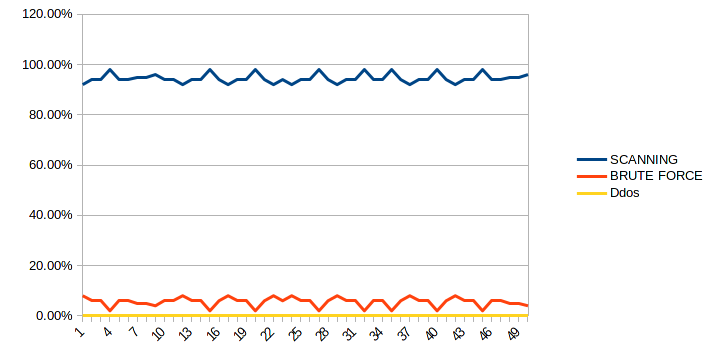
\includegraphics[scale = 0.8]{gambar/scaning}
			\caption{Grafik Deteksi Scanning}
			\label{Grafik Deteksi Scanning}
		\end{figure}
	
	
	Pada pengujian akurasi deteksi \emph{scanning} yang belum dimasukan deteksi paket normal didapatkan hasil rata rata deteksi \emph{scanning} 94.48\%, \emph{brute force} 5.52\% dan \emph{DDoS} 0\% 
	
	Berdasarkan hasil pengujian pada deteksi akurasi \emph{scanning} terdapat \emph{traffik anomali} serangan \emph{brute force} sebesar 5.52\% . Setelah menganalisa traffik \emph{scanning} dengan \emph{wireshark} didapatkan proses \emph{syn / syncronise} pada service \emph{ssh dan ftp } . Hal ini didasarkan ketika proses \emph{scanning} terjadi maka setiap \emph{service} yang aktip akan menerima proses sinkronisasi pada TCP , untuk mengetahui apakah sebuah service aktip atau tidak. 
	
		\newpage
		\noindent
		\textbf{B. Akurasi Serangan \emph{Brute Force}}
	
		Berikut akurasi serangan \emph{Brute Force} tanpa paket normal
		
\begin{table}[H]
	\centering
	\caption{Akurasi Serangan \emph{Brute Force}}
	\label{Akurasi Serangan Brute Force}
	\begin{tabular}{|c|c|c|c|c|}
		\hline
		NOMER        & SCANNING & BRUTE FORCE & DDoS   & KETERANGAN \\ \hline
		1         & 6.00\%   & 94.00\%     & 0.00\% & MEDUSA     \\ \hline
		2         & 10.00\%  & 90.00\%     & 0.00\% & HYDRA      \\ \hline
		3         & 7.00\%   & 93.00\%     & 0.00\% & MEDUSA     \\ \hline
		4         & 7.00\%   & 93.00\%     & 0.00\% & MEDUSA     \\ \hline
		5         & 7.00\%   & 93.00\%     & 0.00\% & ZERO BRUTE \\ \hline
		6         & 6.00\%   & 94.00\%     & 0.00\% & METASPLOIT \\ \hline
		7         & 6.00\%   & 94.00\%     & 0.00\% & NMAP (NSE) \\ \hline
		8         & 7.00\%   & 93.00\%     & 0.00\% & NMAP (NSE) \\ \hline
		9         & 6.00\%   & 94.00\%     & 0.00\% & HYDRA      \\ \hline
		10        & 6.89\%   & 93.11\%     & 0.00\% & MEDUSA     \\ \hline
		11        & 6.00\%   & 94.00\%     & 0.00\% & HYDRA      \\ \hline
		12        & 10.00\%  & 90.00\%     & 0.00\% & MEDUSA     \\ \hline
		13        & 7.00\%   & 93.00\%     & 0.00\% & HYDRA      \\ \hline
		14        & 7.00\%   & 93.00\%     & 0.00\% & MEDUSA     \\ \hline
		15        & 7.00\%   & 93.00\%     & 0.00\% & METASPLOIT \\ \hline
		16        & 6.00\%   & 94.00\%     & 0.00\% & NMAP (NSE) \\ \hline
		17        & 6.00\%   & 94.00\%     & 0.00\% & NMAP (NSE) \\ \hline
		18        & 7.00\%   & 93.00\%     & 0.00\% & HYDRA      \\ \hline
		19        & 6.00\%   & 94.00\%     & 0.00\% & MEDUSA     \\ \hline
		20        & 6.89\%   & 93.11\%     & 0.00\% & NMAP (NSE) \\ \hline
		21        & 7.00\%   & 93.00\%     & 0.00\% & HYDRA      \\ \hline
		22        & 6.00\%   & 94.00\%     & 0.00\% & MEDUSA     \\ \hline
		23        & 6.00\%   & 94.00\%     & 0.00\% & METASPLOIT \\ \hline
		24        & 7.00\%   & 93.00\%     & 0.00\% & MEDUSA     \\ \hline
		25        & 6.00\%   & 94.00\%     & 0.00\% & METASPLOIT \\ \hline
		
			\end{tabular}
	\end{table}

\begin{table}[H]
	\centering

	\begin{tabular}{|c|c|c|c|c|}
		\hline
		NOMER        & SCANNING & BRUTE FORCE & DDoS   & KETERANGAN \\ \hline
		26        & 6.89\%   & 93.11\%     & 0.00\% & METASPLOIT \\ \hline
		27        & 6.00\%   & 94.00\%     & 0.00\% & NMAP (NSE) \\ \hline
		28        & 10.00\%  & 90.00\%     & 0.00\% & NMAP (NSE) \\ \hline
		29        & 7.00\%   & 93.00\%     & 0.00\% & HYDRA      \\ \hline
		30        & 6.00\%   & 94.00\%     & 0.00\% & MEDUSA     \\ \hline
		31        & 7.00\%   & 93.00\%     & 0.00\% & HYDRA      \\ \hline
		32        & 6.00\%   & 94.00\%     & 0.00\% & MEDUSA     \\ \hline
		33        & 6.89\%   & 93.11\%     & 0.00\% & HYDRA      \\ \hline
		34        & 6.00\%   & 94.00\%     & 0.00\% & MEDUSA     \\ \hline
		35        & 10.00\%  & 90.00\%     & 0.00\% & METASPLOIT \\ \hline
		36        & 7.00\%   & 93.00\%     & 0.00\% & NMAP (NSE) \\ \hline
		37        & 6.00\%   & 94.00\%     & 0.00\% & NMAP (NSE) \\ \hline
		38        & 6.00\%   & 94.00\%     & 0.00\% & HYDRA      \\ \hline
		39        & 7.00\%   & 93.00\%     & 0.00\% & HYDRA      \\ \hline
		40        & 6.00\%   & 94.00\%     & 0.00\% & MEDUSA     \\ \hline
		41        & 6.89\%   & 93.11\%     & 0.00\% & METASPLOIT \\ \hline
		42        & 7.00\%   & 93.00\%     & 0.00\% & NMAP (NSE) \\ \hline
		43        & 6.00\%   & 94.00\%     & 0.00\% & NMAP (NSE) \\ \hline
		44        & 6.00\%   & 94.00\%     & 0.00\% & HYDRA      \\ \hline
		45        & 7.00\%   & 93.00\%     & 0.00\% & MEDUSA     \\ \hline
		46        & 6.00\%   & 94.00\%     & 0.00\% & NMAP (NSE) \\ \hline
		47        & 6.89\%   & 93.11\%     & 0.00\% & HYDRA      \\ \hline
		48        & 6.00\%   & 94.00\%     & 0.00\% & MEDUSA     \\ \hline
		49        & 10.00\%  & 90.00\%     & 0.00\% & METASPLOIT \\ \hline
		50        & 7.00\%   & 93.00\%     & 0.00\% & MEDUSA     \\ \hline
		RATA-RATA & 7.00\%  & 93.00\%      & 0.00\% &            \\ \hline
	\end{tabular}
\end{table}
	\begin{figure}[H]
		\centering
		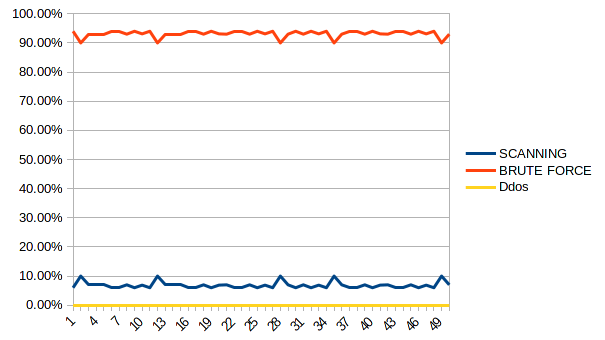
\includegraphics[scale= 0.85]{gambar/brute}
		\caption{Grafik Deteksi \emph{Brute Force} Tanpa Paket Normal}
		\label{Grafik Deteksi Brute Force Tanpa Paket Normal}
	\end{figure}
	
	
	
	Pada pengujian akurasi deteksi \emph{scanning} yang belum dimasukan deteksi paket normal didapatkan hasil rata rata deteksi \emph{scanning} 6.85\%, \emph{brute force} 93.15\% dan \emph{DDoS} 0\% 
	
	Sama halnya dengan hasil pengujian deteksi akurasi \emph{scanning} akan ditemukan \emph{anomali traffik } serangan \emph{brute force} sebesar 6.85\%. Hal ini dikarenakan ketikana akan melakukan \emph{brute force} pada service yang akan di serangan , dalam kasus ini dilakukan serangan pada \emph{service ssh}, setiap 5 detik (setingan default hydra yang digunakan untuk brute force) akan melakukan syncronisasi yang membawa payload \emph{traffik scanning} hal ini yang menyebabkan terjadinya serangan \emph{scanning} pada serangan \emph{brute force}
	
		
		
		
		\newpage
		\noindent
		\textbf{C. Akurasi Deteksi DDoS}
		
				Berikut akurasi serangan \emph{DDoS} tanpa paket normal
		
\begin{table}[H]
	\centering
	\caption{Akurasi Serangan DDoS}
	\label{Akurasi Serangan DDoS}
	\begin{tabular}{|c|c|c|c|c|}
		\hline
		NOMER        & SCANNING & BRUTE FORCE & DDoS    & KETERANGAN \\ \hline
		1         & 2.00\%   & 0.00\%      & 98.00\% & METASPLOIT \\ \hline
		2         & 3.00\%   & 0.00\%      & 97.00\% & METASPLOIT \\ \hline
		3         & 2.00\%   & 0.00\%      & 98.00\% & SLOWLORIS  \\ \hline
		4         & 2.00\%   & 0.00\%      & 98.00\% & PYLoris    \\ \hline
		5         & 3.00\%   & 0.00\%      & 97.00\% & HULK       \\ \hline
		6         & 2.00\%   & 0.00\%      & 98.00\% & HULK       \\ \hline
		7         & 2.00\%   & 0.00\%      & 98.00\% & TCP FLOOD  \\ \hline
		8         & 2.00\%   & 0.00\%      & 98.00\% & METASPLOIT \\ \hline
		9         & 2.00\%   & 0.00\%      & 98.00\% & METASPLOIT \\ \hline
		10        & 2.00\%   & 0.00\%      & 98.00\% & SLOWLORIS  \\ \hline
		11        & 2.00\%   & 0.00\%      & 98.00\% & PYLoris    \\ \hline
		12        & 3.00\%   & 0.00\%      & 97.00\% & HULK       \\ \hline
		13        & 2.00\%   & 0.00\%      & 98.00\% & HULK       \\ \hline
		14        & 2.00\%   & 0.00\%      & 98.00\% & SLOWLORIS  \\ \hline
		15        & 3.00\%   & 0.00\%      & 97.00\% & PYLoris    \\ \hline
		16        & 2.00\%   & 0.00\%      & 98.00\% & HULK       \\ \hline
		17        & 2.00\%   & 0.00\%      & 98.00\% & HULK       \\ \hline
		18        & 2.00\%   & 0.00\%      & 98.00\% & TCP FLOOD  \\ \hline
		19        & 2.00\%   & 0.00\%      & 98.00\% & TCP FLOOD  \\ \hline
		20        & 2.00\%   & 0.00\%      & 98.00\% & PYLoris    \\ \hline
		21        & 3.00\%   & 0.00\%      & 97.00\% & HULK       \\ \hline
		22        & 2.00\%   & 0.00\%      & 98.00\% & HULK       \\ \hline
		23        & 2.00\%   & 0.00\%      & 98.00\% & TCP FLOOD  \\ \hline
		24        & 3.00\%   & 0.00\%      & 97.00\% & METASPLOIT \\ \hline
		25        & 2.00\%   & 0.00\%      & 98.00\% & METASPLOIT \\ \hline
			\end{tabular}
	\end{table}
\begin{table}[H]
	\centering

	\begin{tabular}{|c|c|c|c|c|}
		\hline
		NOMER        & SCANNING & BRUTE FORCE & DDoS    & KETERANGAN \\ \hline
		26        & 3.00\%   & 0.00\%      & 97.00\% & SLOWLORIS  \\ \hline
		27        & 2.00\%   & 0.00\%      & 98.00\% & PYLoris    \\ \hline
		28        & 2.00\%   & 0.00\%      & 98.00\% & HULK       \\ \hline
		29        & 3.00\%   & 0.00\%      & 97.00\% & HULK       \\ \hline
		30        & 2.00\%   & 0.00\%      & 98.00\% & SLOWLORIS  \\ \hline
		31        & 2.00\%   & 0.00\%      & 98.00\% & PYLoris    \\ \hline
		32        & 2.00\%   & 0.00\%      & 98.00\% & HULK       \\ \hline
		33        & 2.00\%   & 0.00\%      & 98.00\% & HULK       \\ \hline
		34        & 2.00\%   & 0.00\%      & 98.00\% & HULK       \\ \hline
		35        & 2.00\%   & 0.00\%      & 98.00\% & TCP FLOOD  \\ \hline
		36        & 3.00\%   & 0.00\%      & 97.00\% & METASPLOIT \\ \hline
		37        & 2.00\%   & 0.00\%      & 98.00\% & METASPLOIT \\ \hline
		38        & 2.00\%   & 0.00\%      & 98.00\% & SLOWLORIS  \\ \hline
		39        & 3.00\%   & 0.00\%      & 97.00\% & PYLoris    \\ \hline
		40        & 2.00\%   & 0.00\%      & 98.00\% & METASPLOIT \\ \hline
		41        & 2.00\%   & 0.00\%      & 98.00\% & METASPLOIT \\ \hline
		42        & 2.00\%   & 0.00\%      & 98.00\% & SLOWLORIS  \\ \hline
		43        & 2.00\%   & 0.00\%      & 98.00\% & SLOWLORIS  \\ \hline
		44        & 2.00\%   & 0.00\%      & 98.00\% & PYLoris    \\ \hline
		45        & 3.00\%   & 0.00\%      & 97.00\% & HULK       \\ \hline
		46        & 2.00\%   & 0.00\%      & 98.00\% & HULK       \\ \hline
		47        & 2.00\%   & 0.00\%      & 98.00\% & SLOWLORIS  \\ \hline
		48        & 3.00\%   & 0.00\%      & 97.00\% & TCP FLOOD  \\ \hline
		49        & 2.00\%   & 0.00\%      & 98.00\% & METASPLOIT \\ \hline
		50        & 2.00\%   & 0.00\%      & 98.00\% & METASPLOIT \\ \hline
		RATA-RATA & 2.00\%   & 0.00\%      & 98.00\% &            \\ \hline
	\end{tabular}
\end{table}
	
	\begin{figure}[H]
		\centering
		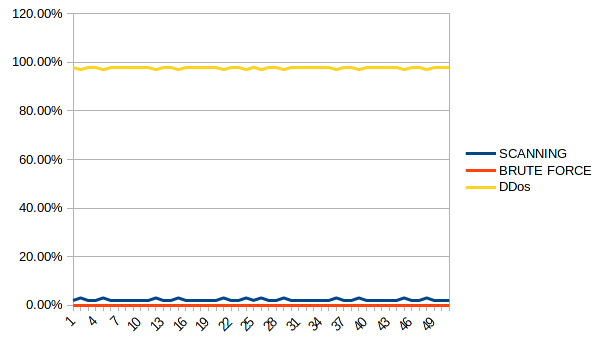
\includegraphics[scale=0.9]{gambar/DDOS}
		\caption{Grafik Deteksi DDoS Tanpa Paket Normal}
		\label{Grafik Deteksi DDoS Tanpa Paket Normal}
	\end{figure}
	
	
	Pada hasil pengujian akurasi serangan deteksi DDoS didapatkan hasil rata-rata deteksi \emph{(scanning)} 2.23\% , \emph{brute force} 0.00 \% dan \emph{DDoS} 97.73\% . 
	
	Pada serangan ini pun ditemukan \emph{traffik anomali} serangan \emph{scanning} hal ini diakibatkan karena pada saat proses  \emph{DDoS} terjadi , service yang sedang dibanjiri \emph{traffik DDoS} secara terus menurus akan melakukan proses \emph{syn/ack} kepada \emph{host} yang melakukan serangan, pada proses itu ada \emph{traffik} yang sama dengan \emph{traffik scanning} 
		
		
		\newpage
		
		\subsection{Skenario Kedua}
				
		Pada scenario ini  akan diuji masing masing akurasi deteksi serangan dengan memasukan \emph{rule} traffik normal,pengujian ini dilakukan sealama 50 kali pengujian
		serangan dimana masing-masing serangan dilakukan secara satu persatu atau terpi-
		sah disamping itu dalam penelitian tugas akhir ini dilukan monitoring penggunaan
		serangan, berikut kami sajikan table dan bagan hasil pengujian dari masing masing akurasi deteksi serangan :
		\newline
		
		
				

		\noindent
		\textbf{A. Akurasi Deteksi Scanning Dengan Memasukan Data Normal}
		
	\begin{table}[H]
		\centering
		\caption{ Akurasi Deteksi Scanning Dengan Memasukan Data Normal}
		\label{ Akurasi Deteksi Scanning Dengan Memasukan Data Normal}
		\begin{tabular}{|c|c|c|c|c|l|}
			\hline
			NOMER        & SCANNING & \begin{tabular}[c]{@{}l@{}}BRUTE \\ FORCE\end{tabular} & DDoS   & NORMAL & KETERANGAN   \\ \hline
			1         & 90.00\%  & 8.00\%      & 0.00\% & 2\%    & NMAP         \\ \hline
			2         & 91.00\%  & 6.00\%      & 0.00\% & 3\%    & NMAP         \\ \hline
			3         & 92.00\%  & 6.00\%      & 0.00\% & 2\%    & METASPLOIT   \\ \hline
			4         & 90.00\%  & 8.00\%      & 0.00\% & 2\%    & TCP SCANNING \\ \hline
			5         & 91.00\%  & 6.00\%      & 0.00\% & 3\%    & NESSUS       \\ \hline
			6         & 92.00\%  & 6.00\%      & 0.00\% & 2\%    & NESSUS       \\ \hline
			7         & 90.00\%  & 8.00\%      & 0.00\% & 2\%    & NMAP         \\ \hline
			8         & 91.00\%  & 6.00\%      & 0.00\% & 3\%    & METASPLOIT   \\ \hline
			9         & 92.00\%  & 6.00\%      & 0.00\% & 2\%    & METASPLOIT   \\ \hline
			10        & 90.00\%  & 8.00\%      & 0.00\% & 2\%    & TCP SCANNING \\ \hline
			11        & 88.00\%  & 8.00\%      & 0.00\% & 4\%    & NESSUS       \\ \hline
			12        & 90.00\%  & 6.00\%      & 0.00\% & 4\%    & TCP SCANNING \\ \hline
			13        & 91.00\%  & 6.00\%      & 0.00\% & 3\%    & METASPLOIT   \\ \hline
			14        & 92.00\%  & 6.00\%      & 0.00\% & 2\%    & METASPLOIT   \\ \hline
			15        & 90.00\%  & 8.00\%      & 0.00\% & 2\%    & TCP SCANNING \\ \hline
			16        & 88.00\%  & 8.00\%      & 0.00\% & 4\%    & NESSUS       \\ \hline
			17        & 90.00\%  & 6.00\%      & 0.00\% & 4\%    & NESSUS       \\ \hline
			18        & 88.00\%  & 8.00\%      & 0.00\% & 4\%    & NMAP         \\ \hline
			19        & 90.00\%  & 6.00\%      & 0.00\% & 4\%    & METASPLOIT   \\ \hline
				\end{tabular}
		\end{table}
	
		\begin{table}[H]
		\centering

		\begin{tabular}{|c|c|c|c|c|l|}
			\hline
			NOMER        & SCANNING & \begin{tabular}[c]{@{}l@{}}BRUTE \\ FORCE\end{tabular} & DDoS   & NORMAL & KETERANGAN   \\ \hline
	
			
			20        & 91.00\%  & 6.00\%      & 0.00\% & 3\%    & METASPLOIT   \\ \hline
			21        & 92.00\%  & 6.00\%      & 0.00\% & 2\%    & TCP SCANNING \\ \hline
			22        & 90.00\%  & 8.00\%      & 0.00\% & 2\%    & NESSUS       \\ \hline
			23        & 88.00\%  & 8.00\%      & 0.00\% & 4\%    & TCP SCANNING \\ \hline
			24        & 90.00\%  & 6.00\%      & 0.00\% & 4\%    & METASPLOIT   \\ \hline
			25        & 90.00\%  & 8.00\%      & 0.00\% & 2\%    & NESSUS       \\ \hline
			26        & 88.00\%  & 8.00\%      & 0.00\% & 4\%    & TCP SCANNING \\ \hline
			27        & 90.00\%  & 6.00\%      & 0.00\% & 4\%    & METASPLOIT   \\ \hline
			28        & 88.00\%  & 8.00\%      & 0.00\% & 4\%    & METASPLOIT   \\ \hline
			29        & 90.00\%  & 6.00\%      & 0.00\% & 4\%    & TCP SCANNING \\ \hline
			30        & 91.00\%  & 6.00\%      & 0.00\% & 3\%    & NESSUS       \\ \hline
			31        & 92.00\%  & 6.00\%      & 0.00\% & 2\%    & NESSUS       \\ \hline
			32        & 90.00\%  & 8.00\%      & 0.00\% & 2\%    & NMAP         \\ \hline
			33        & 90.00\%  & 6.00\%      & 0.00\% & 4\%    & METASPLOIT   \\ \hline
			34        & 91.00\%  & 6.00\%      & 0.00\% & 3\%    & METASPLOIT   \\ \hline
			35        & 92.00\%  & 6.00\%      & 0.00\% & 2\%    & TCP SCANNING \\ \hline
			36        & 90.00\%  & 8.00\%      & 0.00\% & 2\%    & NESSUS       \\ \hline
			37        & 88.00\%  & 8.00\%      & 0.00\% & 4\%    & TCP SCANNING \\ \hline
			38        & 90.00\%  & 6.00\%      & 0.00\% & 4\%    & METASPLOIT   \\ \hline
			39        & 90.00\%  & 8.00\%      & 0.00\% & 2\%    & METASPLOIT   \\ \hline
			40        & 88.00\%  & 8.00\%      & 0.00\% & 4\%    & TCP SCANNING \\ \hline
			41        & 90.00\%  & 6.00\%      & 0.00\% & 4\%    & NESSUS       \\ \hline
			42        & 90.00\%  & 6.00\%      & 0.00\% & 4\%    & NESSUS       \\ \hline
			43        & 91.00\%  & 6.00\%      & 0.00\% & 3\%    & NMAP         \\ \hline
			44        & 92.00\%  & 6.00\%      & 0.00\% & 2\%    & METASPLOIT   \\ \hline
			45        & 90.00\%  & 8.00\%      & 0.00\% & 2\%    & METASPLOIT   \\ \hline
			46        & 88.00\%  & 8.00\%      & 0.00\% & 4\%    & TCP SCANNING \\ \hline
			47        & 90.00\%  & 6.00\%      & 0.00\% & 4\%    & NESSUS       \\ \hline
			48        & 90.00\%  & 8.00\%      & 0.00\% & 2\%    & TCP SCANNING \\ \hline
			49        & 88.00\%  & 8.00\%      & 0.00\% & 4\%    & METASPLOIT   \\ \hline
			50        & 90.00\%  & 6.00\%      & 0.00\% & 4\%    & NMAP         \\ \hline
			RATA-RATA & 90.08\%  & 6.88\%      & 0.00\% & 3.04\% &              \\ \hline
		\end{tabular}
	\end{table}
	
	
	
	\begin{figure}[H]
		\centering
		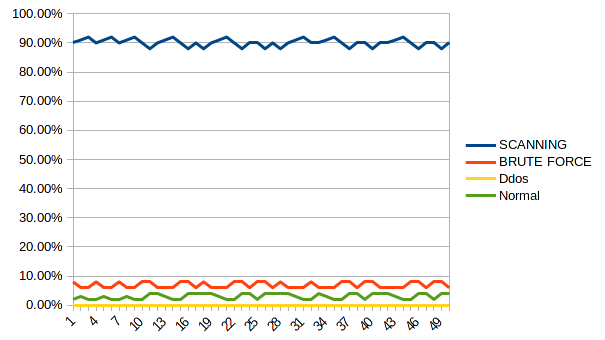
\includegraphics[scale=0.9]{gambar/ddosnormal}
		\caption{Grafik Deteksi Scanning  Dengan Paket Normal}
		\label{Grafik Deteksi Scanning  Dengan Paket Normal}
	\end{figure}
	
	
	Pada pengujian yang ini didapatkan hasil akurasi \emph{scanning} 90.08\% \emph{brute force} 6.88\% \emph{DDoS} 0.0\% dan paket normal 3.04 \%.
		
	Sama halnya dengan peengujian sebelumnya akan terdeteksi juga serangan \emph{brute force}
	
	Setalah memasukan deteksi \emph{traffik} normal akan didapatkan pada serangan \emph{scanning} sebesar 3.04\% hal itu diakibatkan kerana proses \emph{echo-reply} paket \emph{icmp}
	

		\newpage
		\noindent
		\textbf{B. Akurasi Deteksi Brute Force Dengan Memasukan Data Normal}
		
\begin{table}[H]
	\centering
	\caption{Akurasi Deteksi Brute Force Dengan Memasukan Data Normal}
	\label{Akurasi Deteksi Brute Force Dengan Memasukan Data Normal}
	\begin{tabular}{|c|c|c|c|c|l|}
		\hline
		NOMER        & SCANNING & \begin{tabular}[c]{@{}l@{}}BRUTE \\ FORCE\end{tabular} & DDoS   & NORMAL & KETERANGAN   \\ \hline
		1         & 6.00\%   & 88.00\%     & 0.00\% & 6\%    & MEDUSA     \\ \hline
		2         & 6.00\%   & 87.00\%     & 0.00\% & 7\%    & HYDRA      \\ \hline
		3         & 7.00\%   & 88.00\%     & 0.00\% & 5\%    & MEDUSA     \\ \hline
		4         & 7.00\%   & 87.00\%     & 0.00\% & 6\%    & MEDUSA     \\ \hline
		5         & 7.00\%   & 87.00\%     & 0.00\% & 6\%    & ZERO BRUTE \\ \hline
		6         & 6.00\%   & 86.00\%     & 0.00\% & 8\%    & METASPLOIT \\ \hline
		7         & 6.00\%   & 88.00\%     & 0.00\% & 6\%    & NMAP (NSE) \\ \hline
		8         & 6.00\%   & 87.00\%     & 0.00\% & 7\%    & NMAP (NSE) \\ \hline
		9         & 7.00\%   & 88.00\%     & 0.00\% & 5\%    & HYDRA      \\ \hline
		10        & 7.00\%   & 87.00\%     & 0.00\% & 6\%    & MEDUSA     \\ \hline
		11        & 7.00\%   & 87.00\%     & 0.00\% & 6\%    & HYDRA      \\ \hline
		12        & 6.00\%   & 86.00\%     & 0.00\% & 8\%    & MEDUSA     \\ \hline
		13        & 7.00\%   & 87.00\%     & 0.00\% & 6\%    & HYDRA      \\ \hline
		14        & 7.00\%   & 87.00\%     & 0.00\% & 6\%    & MEDUSA     \\ \hline
		15        & 6.00\%   & 86.00\%     & 0.00\% & 8\%    & METASPLOIT \\ \hline
		16        & 6.00\%   & 88.00\%     & 0.00\% & 6\%    & NMAP (NSE) \\ \hline
		17        & 6.00\%   & 87.00\%     & 0.00\% & 7\%    & NMAP (NSE) \\ \hline
		18        & 7.00\%   & 88.00\%     & 0.00\% & 5\%    & HYDRA      \\ \hline
		19        & 7.00\%   & 87.00\%     & 0.00\% & 6\%    & MEDUSA     \\ \hline
		20        & 6.00\%   & 88.00\%     & 0.00\% & 6\%    & NMAP (NSE) \\ \hline
		21        & 6.00\%   & 87.00\%     & 0.00\% & 7\%    & HYDRA      \\ \hline
		22        & 7.00\%   & 88.00\%     & 0.00\% & 5\%    & MEDUSA     \\ \hline
		23        & 7.00\%   & 87.00\%     & 0.00\% & 6\%    & METASPLOIT \\ \hline
		24        & 7.00\%   & 87.00\%     & 0.00\% & 6\%    & MEDUSA     \\ \hline
		25        & 6.00\%   & 86.00\%     & 0.00\% & 8\%    & METASPLOIT \\ \hline
	\end{tabular}
\end{table}
		
\begin{table}[H]
	\centering

	\begin{tabular}{|c|c|c|c|c|l|}
		\hline
		NOMER        & SCANNING & \begin{tabular}[c]{@{}l@{}}BRUTE \\ FORCE\end{tabular} & DDoS   & NORMAL & KETERANGAN   \\ \hline
		26        & 6.00\%   & 88.00\%     & 0.00\% & 6\%    & METASPLOIT \\ \hline
		27        & 6.00\%   & 87.00\%     & 0.00\% & 7\%    & NMAP (NSE) \\ \hline
		28        & 7.00\%   & 88.00\%     & 0.00\% & 5\%    & NMAP (NSE) \\ \hline
		29        & 7.00\%   & 87.00\%     & 0.00\% & 6\%    & HYDRA      \\ \hline
		30        & 7.00\%   & 87.00\%     & 0.00\% & 6\%    & MEDUSA     \\ \hline
		31        & 6.00\%   & 86.00\%     & 0.00\% & 8\%    & HYDRA      \\ \hline
		32        & 7.00\%   & 87.00\%     & 0.00\% & 6\%    & MEDUSA     \\ \hline
		33        & 7.00\%   & 87.00\%     & 0.00\% & 6\%    & HYDRA      \\ \hline
		34        & 6.00\%   & 86.00\%     & 0.00\% & 8\%    & MEDUSA     \\ \hline
		35        & 6.00\%   & 88.00\%     & 0.00\% & 6\%    & METASPLOIT \\ \hline
		36        & 6.00\%   & 87.00\%     & 0.00\% & 7\%    & NMAP (NSE) \\ \hline
		37        & 7.00\%   & 88.00\%     & 0.00\% & 5\%    & NMAP (NSE) \\ \hline
		38        & 7.00\%   & 87.00\%     & 0.00\% & 6\%    & HYDRA      \\ \hline
		39        & 7.00\%   & 87.00\%     & 0.00\% & 6\%    & HYDRA      \\ \hline
		40        & 6.00\%   & 86.00\%     & 0.00\% & 8\%    & MEDUSA     \\ \hline
		41        & 7.00\%   & 87.00\%     & 0.00\% & 6\%    & METASPLOIT \\ \hline
		42        & 7.00\%   & 87.00\%     & 0.00\% & 6\%    & NMAP (NSE) \\ \hline
		43        & 6.00\%   & 86.00\%     & 0.00\% & 8\%    & NMAP (NSE) \\ \hline
		44        & 6.00\%   & 88.00\%     & 0.00\% & 6\%    & HYDRA      \\ \hline
		45        & 6.00\%   & 87.00\%     & 0.00\% & 7\%    & MEDUSA     \\ \hline
		46        & 7.00\%   & 88.00\%     & 0.00\% & 5\%    & NMAP (NSE) \\ \hline
		47        & 7.00\%   & 87.00\%     & 0.00\% & 6\%    & HYDRA      \\ \hline
		48        & 6.00\%   & 88.00\%     & 0.00\% & 6\%    & MEDUSA     \\ \hline
		49        & 6.00\%   & 87.00\%     & 0.00\% & 7\%    & METASPLOIT \\ \hline
		50        & 7.00\%   & 88.00\%     & 0.00\% & 5\%    & MEDUSA     \\ \hline
		RATA-RATA & 6.52\%   & 87.15\%     & 0.00\% & 6.33\% &            \\ \hline
	\end{tabular}
\end{table}


\begin{figure}[H]
	\centering
	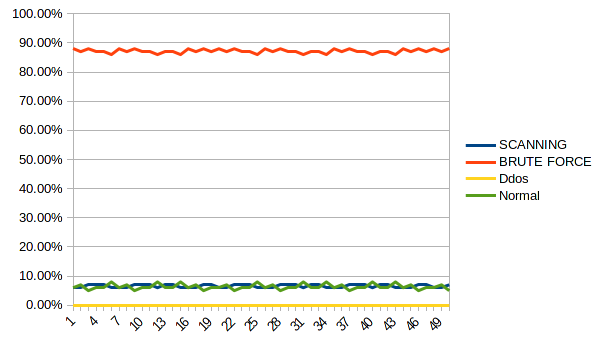
\includegraphics[scale=0.9]{gambar/brutenormal}
	\caption{Grafik Deteksi Brute Force Dengan Paket Normal}
	\label{Grafik Deteksi Brute Force Dengan  Paket Normal}
\end{figure}

	
Pada pengujian yang ini didapatkan hasil akurasi \emph{scanning} 6.52\% \emph{brute force} 87.16\% \emph{DDoS} 0.0\% dan paket normal 6.32 \%.

Sama halnya dengan peengujian sebelumnya akan terdeteksi juga serangan \emph{scanning}

Setalah memasukan deteksi \emph{traffik} normal akan didapatkan pada serangan \emph{scanning} sebesar 6.32\% hal itu diakibatkan kerana proses \emph{echo-reply} paket \emph{icmp}



		\newpage
		\noindent
		\textbf{C. Akurasi Deteksi DDoS Dengan Memasukan Data Normal}
\begin{table}[H]
	\centering
	\caption{Akurasi Deteksi DDoS Dengan Memasukan Data Normal}
	\label{Akurasi Deteksi DDoS Dengan Memasukan Data Normal}
	\begin{tabular}{|c|c|c|c|c|l|}
		\hline
		NOMER        & SCANNING & \begin{tabular}[c]{@{}c@{}}BRUTE \\ FORCE\end{tabular} & DDoS    & NORMAL & KETERANGAN \\ \hline
		1         & 2.00\%   & 0.00\%                                                 & 98.00\% & 0\%    & METASPLOIT \\ \hline
		2         & 3.00\%   & 0.00\%                                                 & 97.00\% & 0\%    & METASPLOIT \\ \hline
		3         & 2.00\%   & 0.00\%                                                 & 96.00\% & 2\%    & SLOWLORIS  \\ \hline
		4         & 2.00\%   & 0.00\%                                                 & 98.00\% & 0\%    & PYLoris    \\ \hline
		5         & 3.00\%   & 0.00\%                                                 & 96.00\% & 1\%    & HULK       \\ \hline
		6         & 2.00\%   & 0.00\%                                                 & 98.00\% & 0\%    & HULK       \\ \hline
		7         & 2.00\%   & 0.00\%                                                 & 98.00\% & 0\%    & TCP FLOOD  \\ \hline
		8         & 2.00\%   & 0.00\%                                                 & 98.00\% & 0\%    & METASPLOIT \\ \hline
		9         & 2.00\%   & 0.00\%                                                 & 98.00\% & 0\%    & METASPLOIT \\ \hline
		10        & 2.00\%   & 0.00\%                                                 & 98.00\% & 0\%    & SLOWLORIS  \\ \hline
		11        & 2.00\%   & 0.00\%                                                 & 98.00\% & 0\%    & PYLoris    \\ \hline
		12        & 3.00\%   & 0.00\%                                                 & 97.00\% & 0\%    & HULK       \\ \hline
		13        & 2.00\%   & 0.00\%                                                 & 98.00\% & 0\%    & HULK       \\ \hline
		14        & 2.00\%   & 0.00\%                                                 & 98.00\% & 0\%    & SLOWLORIS  \\ \hline
		15        & 3.00\%   & 0.00\%                                                 & 97.00\% & 0\%    & PYLoris    \\ \hline
		16        & 2.00\%   & 0.00\%                                                 & 96.00\% & 2\%    & HULK       \\ \hline
		17        & 2.00\%   & 0.00\%                                                 & 98.00\% & 0\%    & HULK       \\ \hline
		18        & 3.00\%   & 0.00\%                                                 & 96.00\% & 1\%    & TCP FLOOD  \\ \hline
		19        & 2.00\%   & 0.00\%                                                 & 98.00\% & 0\%    & TCP FLOOD  \\ \hline
		20        & 2.00\%   & 0.00\%                                                 & 98.00\% & 0\%    & PYLoris    \\ \hline
		21        & 2.00\%   & 0.00\%                                                 & 98.00\% & 0\%    & HULK       \\ \hline
		22        & 2.00\%   & 0.00\%                                                 & 98.00\% & 0\%    & HULK       \\ \hline
		23        & 2.00\%   & 0.00\%                                                 & 98.00\% & 0\%    & TCP FLOOD  \\ \hline
		24        & 2.00\%   & 0.00\%                                                 & 98.00\% & 0\%    & METASPLOIT \\ \hline
		
	\end{tabular}
\end{table}
		
\begin{table}[H]
	\centering
	\begin{tabular}{|c|c|c|c|c|l|}
		\hline
		NO        & SCANNING & \begin{tabular}[c]{@{}c@{}}BRUTE \\ FORCE\end{tabular} & DDoS    & NORMAL & KETERANGAN \\ \hline
		
		25        & 3.00\%   & 0.00\%                                                 & 97.00\% & 0\%    & METASPLOIT \\ \hline
		26        & 2.00\%   & 0.00\%                                                 & 98.00\% & 0\%    & SLOWLORIS  \\ \hline
		27        & 2.00\%   & 0.00\%                                                 & 98.00\% & 0\%    & PYLoris    \\ \hline
		28        & 3.00\%   & 0.00\%                                                 & 97.00\% & 0\%    & HULK       \\ \hline
		29        & 2.00\%   & 0.00\%                                                 & 96.00\% & 2\%    & HULK       \\ \hline
		30        & 2.00\%   & 0.00\%                                                 & 98.00\% & 0\%    & SLOWLORIS  \\ \hline
		31        & 3.00\%   & 0.00\%                                                 & 96.00\% & 1\%    & PYLoris    \\ \hline
		32        & 2.00\%   & 0.00\%                                                 & 98.00\% & 0\%    & HULK       \\ \hline
		33        & 2.00\%   & 0.00\%                                                 & 98.00\% & 0\%    & HULK       \\ \hline
		34        & 2.00\%   & 0.00\%                                                 & 98.00\% & 0\%    & HULK       \\ \hline
		35        & 3.00\%   & 0.00\%                                                 & 96.00\% & 1\%    & TCP FLOOD  \\ \hline
		36        & 2.00\%   & 0.00\%                                                 & 98.00\% & 0\%    & METASPLOIT \\ \hline
		37        & 2.00\%   & 0.00\%                                                 & 98.00\% & 0\%    & METASPLOIT \\ \hline
		38        & 2.00\%   & 0.00\%                                                 & 98.00\% & 0\%    & SLOWLORIS  \\ \hline
		39        & 2.00\%   & 0.00\%                                                 & 98.00\% & 0\%    & PYLoris    \\ \hline
		40        & 2.00\%   & 0.00\%                                                 & 98.00\% & 0\%    & METASPLOIT \\ \hline
		41        & 2.00\%   & 0.00\%                                                 & 98.00\% & 0\%    & METASPLOIT \\ \hline
		42        & 3.00\%   & 0.00\%                                                 & 97.00\% & 0\%    & SLOWLORIS  \\ \hline
		43        & 2.00\%   & 0.00\%                                                 & 98.00\% & 0\%    & SLOWLORIS  \\ \hline
		44        & 2.00\%   & 0.00\%                                                 & 98.00\% & 0\%    & PYLoris    \\ \hline
		45        & 3.00\%   & 0.00\%                                                 & 97.00\% & 0\%    & HULK       \\ \hline
		46        & 2.00\%   & 0.00\%                                                 & 96.00\% & 2\%    & HULK       \\ \hline
		47        & 2.00\%   & 0.00\%                                                 & 98.00\% & 0\%    & SLOWLORIS  \\ \hline
		48        & 3.00\%   & 0.00\%                                                 & 97.00\% & 0\%    & TCP FLOOD  \\ \hline
		49        & 2.00\%   & 0.00\%                                                 & 98.00\% & 0\%    & METASPLOIT \\ \hline
		50        & 2.00\%   & 0.00\%                                                 & 98.00\% & 0\%    & METASPLOIT \\ \hline
		RATA-RATA & 3.00\%   & 0.00\%                                                 & 97.00\% & 0\%    &            \\ \hline
	\end{tabular}
\end{table}





	\begin{figure}[H]
		\centering
		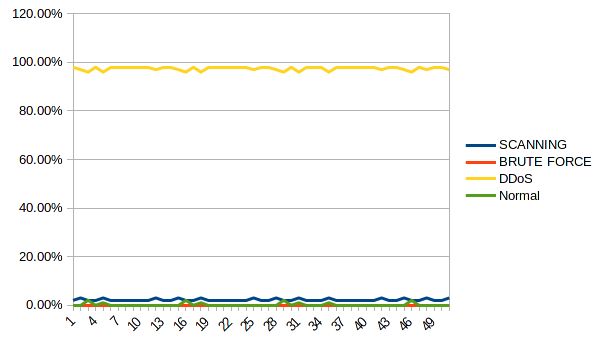
\includegraphics[scale=0.9]{gambar/ddosnormal1}
		\caption{Grafik Deteksi DDoS Dengan Paket Normal}
		\label{Grafik DDos Force Dengan  Paket Normal}
	\end{figure}
	
	
	
	Pada pengujian yang ini didapatkan hasil akurasi \emph{scanning} 2.25\% \emph{brute force} 0.00\% \emph{DDoS} 97.51\% dan paket normal 0.24 \%.
	
	Sama halnya dengan peengujian sebelumnya akan terdeteksi juga serangan \emph{scanning}
	
	Setalah memasukan deteksi \emph{traffik} normal akan didapatkan pada serangan \emph{scanning} sebesar 0.24\% hal itu diakibatkan kerana proses \emph{echo-reply} paket \emph{icmp}
	
	
	
	\newpage
	\subsection{Skenario Ketiga}
	Pada pengujian di skenario ini , akan ditunjukan perbandingan akurasi deteksi antara menggunakan paket normal dan tidak menggunakan paket normal 
	
	\noindent
	\textbf{A. Perbandingan Akurasi Deteksi Scanning }
	
	\begin{table}[H]
		\centering
		\caption{ Perbandingan Akurasi Deteksi Scanning}
		\label{Perbandingan Akurasi Deteksi Scanning}
		\begin{tabular}{|l|l|l|l|l|l|}
			\hline
no & \multicolumn{1}{c|}{\begin{tabular}[c]{@{}c@{}}Scanning tanpa\\ paket normal\end{tabular}} & \multicolumn{1}{c|}{\begin{tabular}[c]{@{}c@{}}Scanning dengan \\ paket normal\end{tabular}} & no & \multicolumn{1}{c|}{\begin{tabular}[c]{@{}c@{}}Scanning tanpa \\ paket normal\end{tabular}} & \multicolumn{1}{c|}{\begin{tabular}[c]{@{}c@{}}Scanning dengan \\ paket normal\end{tabular}} \\ \hline

			1  & 92.00\%                                                               & 90.00\%                                                                 & 26 & 94.00\%                                                                & 88.00\%                                                                 \\ \hline
			2  & 94.00\%                                                               & 91.00\%                                                                 & 27 & 98.00\%                                                                & 90.00\%                                                                 \\ \hline
			3  & 94.00\%                                                               & 92.00\%                                                                 & 28 & 94.00\%                                                                & 88.00\%                                                                 \\ \hline
			4  & 98.00\%                                                               & 90.00\%                                                                 & 29 & 92.00\%                                                                & 90.00\%                                                                 \\ \hline
			5  & 94.00\%                                                               & 91.00\%                                                                 & 30 & 94.00\%                                                                & 91.00\%                                                                 \\ \hline
			6  & 94.00\%                                                               & 92.00\%                                                                 & 31 & 94.00\%                                                                & 92.00\%                                                                 \\ \hline
			7  & 95.00\%                                                               & 90.00\%                                                                 & 32 & 98.00\%                                                                & 90.00\%                                                                 \\ \hline
			8  & 95.00\%                                                               & 91.00\%                                                                 & 33 & 94.00\%                                                                & 90.00\%                                                                 \\ \hline
			9  & 96.00\%                                                               & 92.00\%                                                                 & 34 & 94.00\%                                                                & 91.00\%                                                                 \\ \hline
			10 & 94.00\%                                                               & 90.00\%                                                                 & 35 & 98.00\%                                                                & 92.00\%                                                                 \\ \hline
			11 & 94.00\%                                                               & 88.00\%                                                                 & 36 & 94.00\%                                                                & 90.00\%                                                                 \\ \hline
			12 & 92.00\%                                                               & 90.00\%                                                                 & 37 & 92.00\%                                                                & 88.00\%                                                                 \\ \hline
			13 & 94.00\%                                                               & 91.00\%                                                                 & 38 & 94.00\%                                                                & 90.00\%                                                                 \\ \hline
			14 & 94.00\%                                                               & 92.00\%                                                                 & 39 & 94.00\%                                                                & 90.00\%                                                                 \\ \hline
			15 & 98.00\%                                                               & 90.00\%                                                                 & 40 & 98.00\%                                                                & 88.00\%                                                                 \\ \hline
			16 & 94.00\%                                                               & 88.00\%                                                                 & 41 & 94.00\%                                                                & 90.00\%                                                                 \\ \hline
			17 & 92.00\%                                                               & 90.00\%                                                                 & 42 & 92.00\%                                                                & 90.00\%                                                                 \\ \hline
			18 & 94.00\%                                                               & 88.00\%                                                                 & 43 & 94.00\%                                                                & 91.00\%                                                                 \\ \hline
			19 & 94.00\%                                                               & 90.00\%                                                                 & 44 & 94.00\%                                                                & 92.00\%                                                                 \\ \hline
			20 & 98.00\%                                                               & 91.00\%                                                                 & 45 & 98.00\%                                                                & 90.00\%                                                                 \\ \hline
			21 & 94.00\%                                                               & 92.00\%                                                                 & 46 & 94.00\%                                                                & 88.00\%                                                                 \\ \hline
			22 & 92.00\%                                                               & 90.00\%                                                                 & 47 & 94.00\%                                                                & 90.00\%                                                                 \\ \hline
			23 & 94.00\%                                                               & 88.00\%                                                                 & 48 & 95.00\%                                                                & 90.00\%                                                                 \\ \hline
			24 & 92.00\%                                                               & 90.00\%                                                                 & 49 & 95.00\%                                                                & 88.00\%                                                                 \\ \hline
			25 & 94.00\%                                                               & 90.00\%                                                                 & 50 & 96.00\%                                                                & 90.00\%                                                                 \\ \hline
			&                                                                       & \multicolumn{2}{l|}{rata - rata}                                             & 94.48\%                                                                & 90.08\%                                                                 \\ \hline
		\end{tabular}
	\end{table}

\begin{figure}[H]
	\centering
	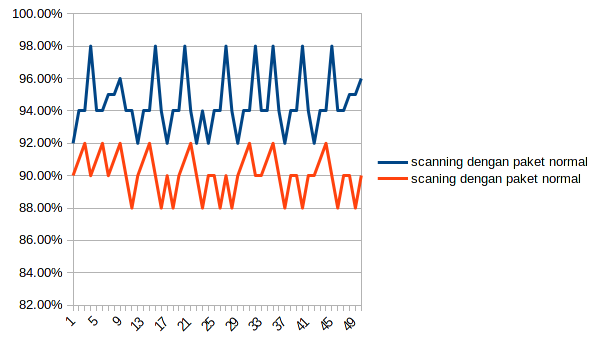
\includegraphics[scale=0.8]{gambar/pscanning}
	\caption{Perbandinan Akurasi Deteksi Scanning}
	\label{Perbandinan Akurasi Deteksi Scanning}
\end{figure}

Pada hasil perbandingan ini didapatkan hasil \emph{(scanning)} tanpa paket normal 94.48\% dan dengan paket normal 90.08\%. Seperti hasil penelitian pada skenario kedua hasil yang didapatkan pada hasil \emph{scanning} tanpa paket normal lebih besar dengan \emph{scanning} yang menggunakan paket normal . Hal ini diakibatkan karena serangan \emph{scanning} memerlukan echo-replay terhadap target

\newpage
\noindent
\textbf{B. Perbandingan Akurasi Deteksi Brute Force }

\begin{table}[H]
	\centering
	\caption{Perbandingan Akurasi Deteksi Brute Force}
	\label{Perbandingan Akurasi Deteksi Brute Force}
	\begin{tabular}{|l|l|l|l|l|l|}
		\hline
		no & \multicolumn{1}{c|}{\begin{tabular}[c]{@{}c@{}}Brute force tanpa\\ paket normal\end{tabular}} & \multicolumn{1}{c|}{\begin{tabular}[c]{@{}c@{}}Brute force dengan \\ paket normal\end{tabular}} & no & \multicolumn{1}{c|}{\begin{tabular}[c]{@{}c@{}}Brute forcetanpa \\ paket normal\end{tabular}} & \multicolumn{1}{c|}{\begin{tabular}[c]{@{}c@{}}Brute force dengan\\  paket normal\end{tabular}} \\ \hline
		1  & 94.00\%                                                                                       & 88.00\%                                                                                         & 26 & 93.11\%                                                                                       & 88.00\%                                                                                         \\ \hline
		2  & 90.00\%                                                                                       & 87.00\%                                                                                         & 27 & 94.00\%                                                                                       & 87.00\%                                                                                         \\ \hline
		3  & 93.00\%                                                                                       & 88.00\%                                                                                         & 28 & 90.00\%                                                                                       & 88.00\%                                                                                         \\ \hline
		4  & 93.00\%                                                                                       & 87.00\%                                                                                         & 29 & 93.00\%                                                                                       & 87.00\%                                                                                         \\ \hline
		5  & 93.00\%                                                                                       & 87.00\%                                                                                         & 30 & 94.00\%                                                                                       & 87.00\%                                                                                         \\ \hline
		6  & 94.00\%                                                                                       & 86.00\%                                                                                         & 31 & 93.00\%                                                                                       & 86.00\%                                                                                         \\ \hline
		7  & 94.00\%                                                                                       & 88.00\%                                                                                         & 32 & 94.00\%                                                                                       & 87.00\%                                                                                         \\ \hline
		8  & 93.00\%                                                                                       & 87.00\%                                                                                         & 33 & 93.11\%                                                                                       & 87.00\%                                                                                         \\ \hline
		9  & 94.00\%                                                                                       & 88.00\%                                                                                         & 34 & 94.00\%                                                                                       & 86.00\%                                                                                         \\ \hline
		10 & 93.11\%                                                                                       & 87.00\%                                                                                         & 35 & 90.00\%                                                                                       & 88.00\%                                                                                         \\ \hline
		11 & 94.00\%                                                                                       & 87.00\%                                                                                         & 36 & 93.00\%                                                                                       & 87.00\%                                                                                         \\ \hline
		12 & 90.00\%                                                                                       & 86.00\%                                                                                         & 37 & 94.00\%                                                                                       & 88.00\%                                                                                         \\ \hline
		13 & 93.00\%                                                                                       & 87.00\%                                                                                         & 38 & 94.00\%                                                                                       & 87.00\%                                                                                         \\ \hline
		14 & 93.00\%                                                                                       & 87.00\%                                                                                         & 39 & 93.00\%                                                                                       & 87.00\%                                                                                         \\ \hline
		15 & 93.00\%                                                                                       & 86.00\%                                                                                         & 40 & 94.00\%                                                                                       & 86.00\%                                                                                         \\ \hline
		16 & 94.00\%                                                                                       & 88.00\%                                                                                         & 41 & 93.11\%                                                                                       & 87.00\%                                                                                         \\ \hline
		17 & 94.00\%                                                                                       & 87.00\%                                                                                         & 42 & 93.00\%                                                                                       & 87.00\%                                                                                         \\ \hline
		18 & 93.00\%                                                                                       & 88.00\%                                                                                         & 43 & 94.00\%                                                                                       & 86.00\%                                                                                         \\ \hline
		19 & 94.00\%                                                                                       & 87.00\%                                                                                         & 44 & 94.00\%                                                                                       & 88.00\%                                                                                         \\ \hline
		20 & 93.11\%                                                                                       & 88.00\%                                                                                         & 45 & 93.00\%                                                                                       & 87.00\%                                                                                         \\ \hline
		21 & 93.00\%                                                                                       & 87.00\%                                                                                         & 46 & 94.00\%                                                                                       & 88.00\%                                                                                         \\ \hline
		22 & 94.00\%                                                                                       & 88.00\%                                                                                         & 47 & 93.11\%                                                                                       & 87.00\%                                                                                         \\ \hline
		23 & 94.00\%                                                                                       & 87.00\%                                                                                         & 48 & 94.00\%                                                                                       & 88.00\%                                                                                         \\ \hline
		24 & 93.00\%                                                                                       & 87.00\%                                                                                         & 49 & 90.00\%                                                                                       & 87.00\%                                                                                         \\ \hline
		25 & 94.00\%                                                                                       & 86.00\%                                                                                         & 50 & 93.00\%                                                                                       & 88.00\%                                                                                         \\ \hline
		&                                                                                               & \multicolumn{2}{l|}{rata - rata}                                                                     & 93.15\%                                                                                       & 87.16\%                                                                                         \\ \hline
	\end{tabular}
\end{table}



\begin{figure}[H]
	\centering
	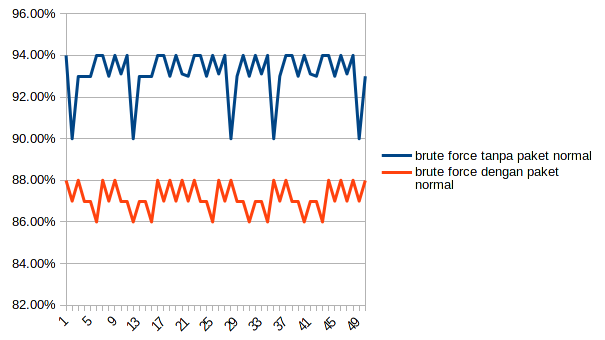
\includegraphics[scale=0.9]{gambar/pbrute}
	\caption{Perbandingan Akurasi Deteksi Brute Force}
	\label{Perbandingan Akurasi Deteksi Brute Force}
\end{figure}

Pada hasil perbandingan ini didapatkan hasil \emph{(brute force)} tanpa paket normal 93.15\% dan dengan paket normal 87.16\%. Seperti hasil penelitian pada skenario kedua hasil yang didapatkan pada hasil \emph{brute force} tanpa paket normal lebih besar dengan \emph{brute force} yang menggunakan paket normal . Hal ini diakibatkan karena serangan \emph{brute force} memerlukan echo-replay terhadap target hal ini juga didapatkan pada serangan \emph{scanning}

	\newpage
	\noindent
	\textbf{C. Perbandingan Akurasi Deteksi DDoS }
	
	
	
	\begin{table}[H]
		\centering
		\caption{ Perbandinan Akurasi Deteksi DDoS}
		\label{ Perbandinan Akurasi Deteksi DDoS}
		\begin{tabular}{|l|l|l|l|l|l|}
			\hline
no & \multicolumn{1}{c|}{\begin{tabular}[c]{@{}c@{}}DDoS tanpa\\ paket normal\end{tabular}} & \multicolumn{1}{c|}{\begin{tabular}[c]{@{}c@{}}DDoS dengan \\ paket normal\end{tabular}} & no & \multicolumn{1}{c|}{\begin{tabular}[c]{@{}c@{}}DDoS tanpa \\ paket normal\end{tabular}} & \multicolumn{1}{c|}{\begin{tabular}[c]{@{}c@{}}DDoS dengan \\ paket normal\end{tabular}} \\ \hline
			1  & 98.00\%                 & 98.00\%                    & 26  & 97.00\%                 & 98.00\%                  \\ \hline
			2  & 97.00\%                 & 97.00\%                    & 27  & 98.00\%                 & 98.00\%                  \\ \hline
			3  & 98.00\%                 & 96.00\%                    & 28  & 98.00\%                 & 97.00\%                  \\ \hline
			4  & 98.00\%                 & 98.00\%                    & 29  & 97.00\%                 & 96.00\%                  \\ \hline
			5  & 97.00\%                 & 96.00\%                    & 30  & 98.00\%                 & 98.00\%                  \\ \hline
			6  & 98.00\%                 & 98.00\%                    & 31  & 98.00\%                 & 96.00\%                  \\ \hline
			7  & 98.00\%                 & 98.00\%                    & 32  & 98.00\%                 & 98.00\%                  \\ \hline
			8  & 98.00\%                 & 98.00\%                    & 33  & 98.00\%                 & 98.00\%                  \\ \hline
			9  & 98.00\%                 & 98.00\%                    & 34  & 98.00\%                 & 98.00\%                  \\ \hline
			10 & 98.00\%                 & 98.00\%                    & 35  & 98.00\%                 & 96.00\%                  \\ \hline
			11 & 98.00\%                 & 98.00\%                    & 36  & 97.00\%                 & 98.00\%                  \\ \hline
			12 & 97.00\%                 & 97.00\%                    & 37  & 98.00\%                 & 98.00\%                  \\ \hline
			13 & 98.00\%                 & 98.00\%                    & 38  & 98.00\%                 & 98.00\%                  \\ \hline
			14 & 98.00\%                 & 98.00\%                    & 39  & 97.00\%                 & 98.00\%                  \\ \hline
			15 & 97.00\%                 & 97.00\%                    & 40  & 98.00\%                 & 98.00\%                  \\ \hline
			16 & 98.00\%                 & 96.00\%                    & 41  & 98.00\%                 & 98.00\%                  \\ \hline
			17 & 98.00\%                 & 98.00\%                    & 42  & 98.00\%                 & 97.00\%                  \\ \hline
			18 & 98.00\%                 & 96.00\%                    & 43  & 98.00\%                 & 98.00\%                  \\ \hline
			19 & 98.00\%                 & 98.00\%                    & 44  & 98.00\%                 & 98.00\%                  \\ \hline
			20 & 98.00\%                 & 98.00\%                    & 45  & 97.00\%                 & 97.00\%                  \\ \hline
			21 & 97.00\%                 & 98.00\%                    & 46  & 98.00\%                 & 96.00\%                  \\ \hline
			22 & 98.00\%                 & 98.00\%                    & 47  & 98.00\%                 & 98.00\%                  \\ \hline
			23 & 98.00\%                 & 98.00\%                    & 48  & 97.00\%                 & 97.00\%                  \\ \hline
			24 & 97.00\%                 & 98.00\%                    & 49  & 98.00\%                 & 98.00\%                  \\ \hline
			25 & 98.00\%                 & 97.00\%                    & 50  & 98.00\%                 & 98.00\%                  \\ \hline
			&                         & \multicolumn{2}{l|}{rata - rata} & 97.76\%                 & 97.52\%                  \\ \hline
		\end{tabular}
	\end{table}
	\newpage
	\begin{figure}[H]
		\centering
		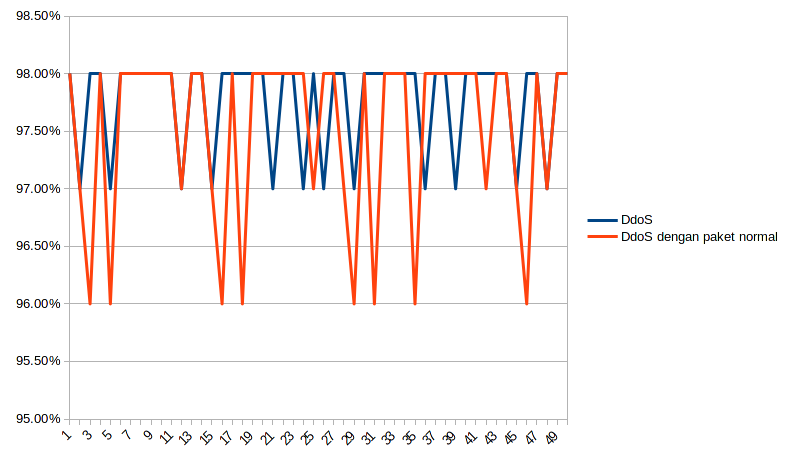
\includegraphics[scale=0.7]{gambar/pddos}
		\caption{Perbandinan Akurasi Deteksi DDoS}
		\label{Perbandinan Akurasi Deteksi DDoS}
	\end{figure}
	
	Pada hasil perbandingan ini didapatkan hasil \emph{DDoS} tanpa paket normal 97.76\% dan dengan paket normal 97.52\%. Seperti hasil penelitian pada skenario kedua hasil yang didapatkan pada hasil \emph{DDoS} tanpa paket normal lebih besar dengan \emph{DDoS} yang menggunakan paket normal . Hal ini diakibatkan karena serangan \emph{DDoS} memerlukan echo-replay, namum pada serangan DDoS didapatkan hasil selisih yang sangat kecil yaitu 0.24\% hal ini karena serangan DDoS mengirim hampir 400 paket perdetik pada tiap sekali melakukan \emph{three-way-handshake (echo-replay)}
	
	\newpage
	\subsection{Skenario Keempat}

	Pada pengujian Skenarion ini akan diuji persentase akurasi berdasarkan banyaknya datasetm jumlah dataset yang diuji akan ditambah sebanyak 10\% dari dataset awal sehingga setiap pengujian akan ditambah sebanyak 500.000 dataset , pengujian ini dilakukan pada sistem operasi Arch linux 64 bit dengan kapasitas Hardware RAM (8 GB) ,
	CPU (2,5 GHz quad core), SSD (read 300 MB, write 350 MB). berikut adalah tabel dan bagan hasil pengujian yang didapatkan:
\newline	


\noindent
\textbf{A. Akurasi Deteksi \emph{(Scanning)} Terhadap Penambahan Dataset}

	\begin{table}[H]
		\centering
		\caption{Akurasi Serangan Terhadap Penambahan Dataset}
		\label{Akurasi Serangan s Terhadap Penambahan Dataset}
		\begin{tabular}{|l|l|l|l|}
			\hline
			jumlah data set & akurasi scanning   & akurasi brute force & akurasi DDoS \\ \hline
			5.000.000       & 94.82\%   & 93.22\%  &  98.22\%     \\ \hline
			5.500.000       & 95.12\%   & 95.32\%  &  98.34\% \\ \hline
			6.000.000       & 96.21\%   & 95.71\%  &  98.51\%  \\ \hline
			6.500.000       & 96.50\%   & 96.12\%  &  98.62\%  \\ \hline
			7.000.000       & 96.70\%   & 96.56\%  &  98.72\%  \\ \hline
		\end{tabular}
	\end{table}


\begin{figure}[H]
	\centering
	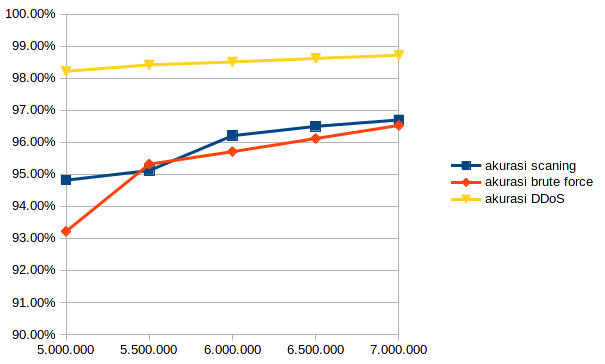
\includegraphics[scale=0.7]{gambar/penambahanDataset}
	\caption{Akurasi Deteksi Serangan Dengan Penambahan Dataset}
	\label{Akurasi Deteksi Serangan Dengan Penambahan Dataset}
\end{figure}

pada pengujian ini hanya mampu melukan pengolahan data pada batas maksimal 7.200.000 s/d 7.300.000 data , jika lebih dari itu aplikasi akan mengalami \emph{force closed}


\newpage
\subsection{Skenarion Kelima}

Pada pengukuran ini dilakukan untuk mengetahui waktu yang dibutuhkan untuk komunikasi antara telegram dan server. Para meter pengukuran ada 3 macan yaitu
sys (waktu yang dibutukan system untuk melakukan compiler program), user (waktu yang dibutuhkan untuk interpreter menjalankan program ), dan real(waktu yang
dibutuhkan untuk menjalankan program sepenuhnya). Pada waktu real ini adalah
waktu yang dibutuhkan unutk komuniasi antara Telegram dan Server cnc , waktu real
berpengaruh pada kecepatan internet . semakin cepat koneksi internet maka semakin
cepat waktu yang dibutuhkan, pada pengujian ini dilakukan pengujian pada kecepatan
internet dengan kecepatan download 900/Kbps dan upload 100/Kbps. Dengan data
table pengujian sebagai berikut :

\begin{table}[H]
	\centering
	\caption{waktu pengiriman telegram-server}
	\label{waktu pengiriman telegram-server}
	\begin{tabular}{|l|l|l|l|l|l|l|l|}
		\hline
		no & \multicolumn{1}{c|}{sys (s)} & \multicolumn{1}{c|}{user (s)} & real (s) & \multicolumn{1}{c|}{no} & sys (s) & user (s) & real (s) \\ \hline
		1  & 0.021                        & 0.33                          & 1.21     & 26                      & 0.023   & 0.31     & 1.24     \\ \hline
		2  & 0.023                        & 0.31                          & 1.24     & 27                      & 0.023   & 0.32     & 1.19     \\ \hline
		3  & 0.021                        & 0.29                          & 1.18     & 28                      & 0.023   & 0.32     & 1.19     \\ \hline
		4  & 0.023                        & 0.32                          & 1.19     & 29                      & 0.021   & 0.33     & 1.21     \\ \hline
		5  & 0.021                        & 0.33                          & 1.21     & 30                      & 0.023   & 0.31     & 1.24     \\ \hline
		6  & 0.023                        & 0.31                          & 1.24     & 31                      & 0.023   & 0.31     & 1.24     \\ \hline
		7  & 0.023                        & 0.31                          & 1.24     & 32                      & 0.023   & 0.32     & 1.19     \\ \hline
		8  & 0.023                        & 0.32                          & 1.19     & 33                      & 0.023   & 0.32     & 1.19     \\ \hline
		9  & 0.023                        & 0.32                          & 1.19     & 34                      & 0.021   & 0.33     & 1.21     \\ \hline
		10 & 0.021                        & 0.33                          & 1.21     & 35                      & 0.023   & 0.31     & 1.24     \\ \hline
		11 & 0.023                        & 0.31                          & 1.24     & 36                      & 0.021   & 0.33     & 1.21     \\ \hline
		12 & 0.023                        & 0.31                          & 1.24     & 37                      & 0.023   & 0.31     & 1.24     \\ \hline
		13 & 0.023                        & 0.32                          & 1.19     & 38                      & 0.021   & 0.29     & 1.18     \\ \hline
		14 & 0.023                        & 0.32                          & 1.19     & 39                      & 0.023   & 0.32     & 1.19     \\ \hline
	\end{tabular}
\end{table}

	
\begin{table}[H]
	\centering
	\begin{tabular}{|l|l|l|l|l|l|l|l|}
		\hline
		no & \multicolumn{1}{c|}{sys (s)} & \multicolumn{1}{c|}{user (s)} & real (s) & \multicolumn{1}{c|}{no} & sys (s) & user (s) & real (s) \\ \hline	
	
		15 & 0.021                        & 0.33                          & 1.21     & 40                      & 0.021   & 0.33     & 1.21     \\ \hline
		16 & 0.023                        & 0.31                          & 1.24     & 41                      & 0.023   & 0.31     & 1.24     \\ \hline
		17 & 0.021                        & 0.33                          & 1.21     & 42                      & 0.023   & 0.32     & 1.19     \\ \hline
		18 & 0.023                        & 0.31                          & 1.24     & 43                      & 0.023   & 0.32     & 1.19     \\ \hline
		19 & 0.021                        & 0.29                          & 1.18     & 44                      & 0.021   & 0.33     & 1.21     \\ \hline
		20 & 0.023                        & 0.32                          & 1.19     & 45                      & 0.023   & 0.31     & 1.24     \\ \hline
		21 & 0.021                        & 0.33                          & 1.21     & 46                      & 0.021   & 0.33     & 1.21     \\ \hline
		22 & 0.023                        & 0.31                          & 1.24     & 47                      & 0.023   & 0.31     & 1.24     \\ \hline
		23 & 0.023                        & 0.31                          & 1.24     & 48                      & 0.023   & 0.31     & 1.24     \\ \hline
		24 & 0.023                        & 0.32                          & 1.19     & 49                      & 0.023   & 0.32     & 1.19     \\ \hline
		25 & 0.023                        & 0.31                          & 1.24     & 50                      & 0.023   & 0.32     & 1.19     \\ \hline
		&                              & \multicolumn{3}{c|}{rata-rata}                                     & 0.0224  & 0.3168   & 1.2132   \\ \hline
	\end{tabular}
\end{table}


\begin{figure}[H]
	\centering
	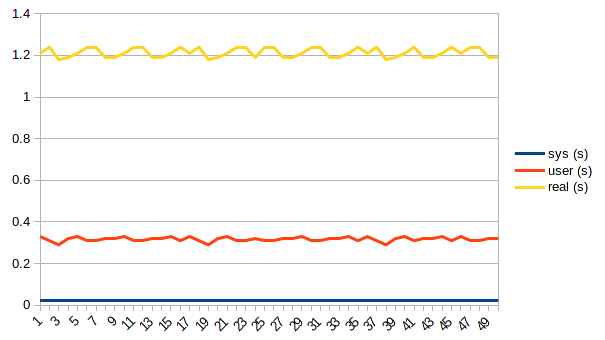
\includegraphics[scale=0.7]{gambar/telegram}
	\caption{waktu pengiriman telegram-server}
	\label{waktu pengiriman telegram-server}
\end{figure}



% Baris ini digunakan untuk membantu dalam melakukan sitasi.
% Karena diapit dengan comment, maka baris ini akan diabaikan
% oleh compiler LaTeX.
\begin{comment}
\bibliography{daftar-pustaka}
\end{comment}



